\documentclass{beamer}
 
\usepackage[francais]{babel}
\usepackage[T1]{fontenc}
\usepackage[utf8]{inputenc}
\usepackage{graphicx, verbatim}
\usepackage{wrapfig}
 
\usetheme{Madrid}
 
\title[L'algorithme Hashlife]{Simulation du jeu de la vie avec l'algorithme Hashlife}
\author[P. COUDERC - D. MAISON]{Pierrick COUDERC - David MAISON}
\institute[u-psud]{Université Paris-Sud}
 
\begin{document}
 
\begin{frame}
\titlepage
\end{frame}



\section{Jeu de la vie}

\begin{frame}{Jeu de la vie}
  \begin{itemize}
  \item Automate cellulaire 2D à deux états
  \item Imaginé par \textbf{John Conway} en 1970
  \end{itemize}

  \medskip

  \begin{center}
    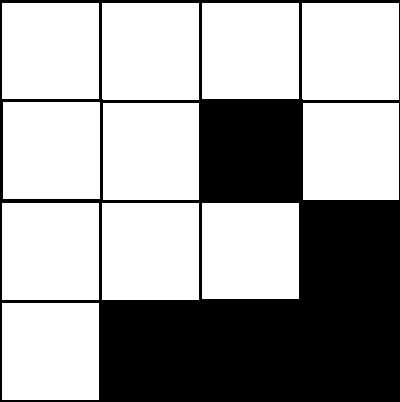
\includegraphics[scale=0.2]{glider.png}

    \textit{Le célèbre glider}
  \end{center}
\end{frame}

\section{L'algorithme Hashlife}

\begin{frame}{L'algorithme Hashlife}
  
  \begin{center}
    Proposé par \textbf{Bill Gosper} dans

    \textit{Exploiting Regularities in Large Cellular Spaces}, 1984

  \end{center}

  \medskip

  Utilité d'Hashlife :
  \begin{itemize}
    \item Simulation à grande échelle de temps et d'espace
    \item Exploitation de la redondance des configurations
  \end{itemize}

\end{frame}

\subsection{Structure de quadtree}

\begin{frame}{Structure de quadtree}

  \begin{columns}[c]
    \begin{column}{2cm}
      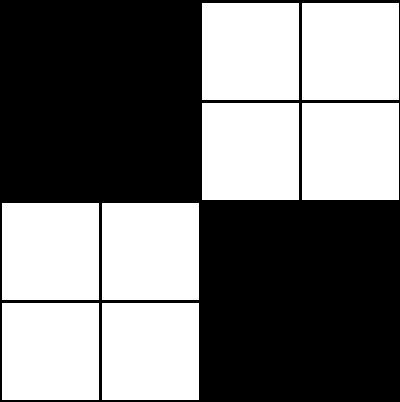
\includegraphics[scale=0.2]{redudancy_ex.png}
    \end{column}

    \begin{column}{6cm}
      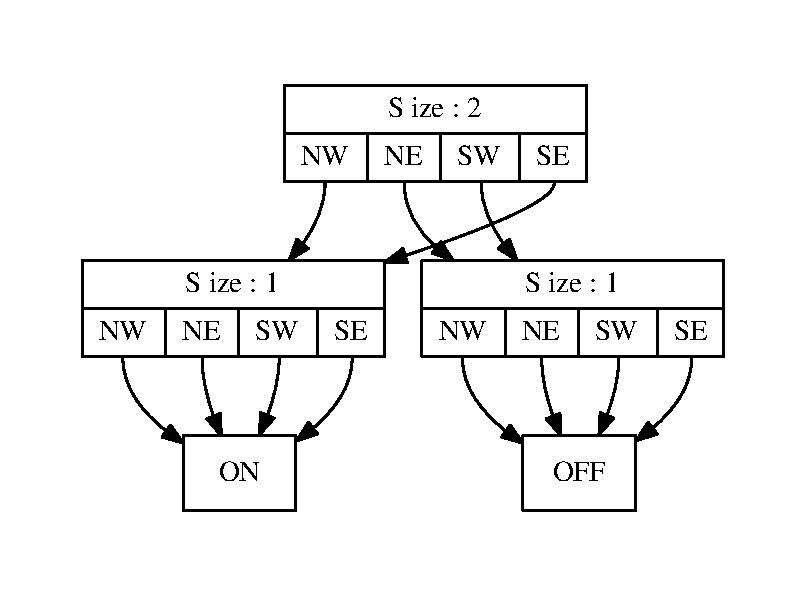
\includegraphics[scale=0.5]{redudancy.pdf}
    \end{column}

  \end{columns}
  
  \begin{center}
    \textit{Une macro-cellule arbitraire et sa représentation sous
      forme de quadtree}
    \end{center}
\end{frame}

\subsection{L'idée centrale de l'algorithme}

\begin{frame}{L'idée centrale de l'algorithme}

\begin{columns}[c]
  \begin{column}{5cm}
    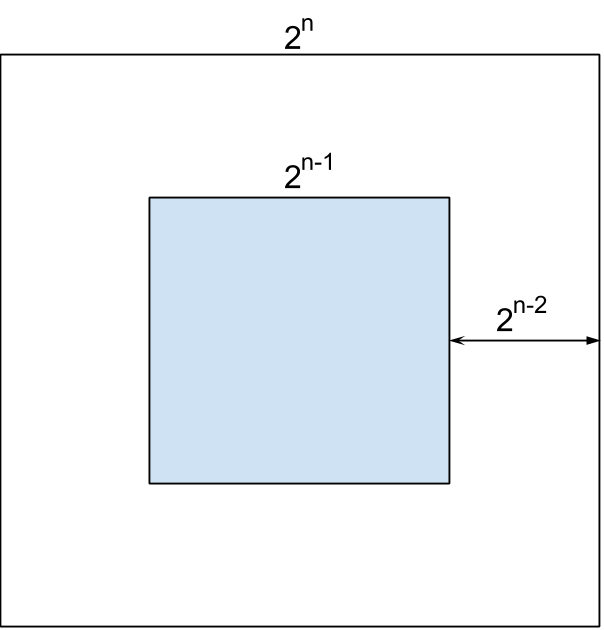
\includegraphics[scale=0.2]{result.png}
  \end{column}
  \begin{column}{5cm}
    La macro-cellule de taille 2\textsuperscript{n-1} ne dépend
    pas de l'extérieur de la cellule de taille 2\textsuperscript{n}
    dans un pas de temps de 2\textsuperscript{n-2}
  \end{column}
\end{columns}

\end{frame}

\subsection{Calcul récursif}

\begin{frame}{Calcul récursif}
  \begin{center}
    Calcul récursif du résultat en quatre étapes 
  \end{center}

  \begin{columns}[c]

    \begin{column}{2cm}
      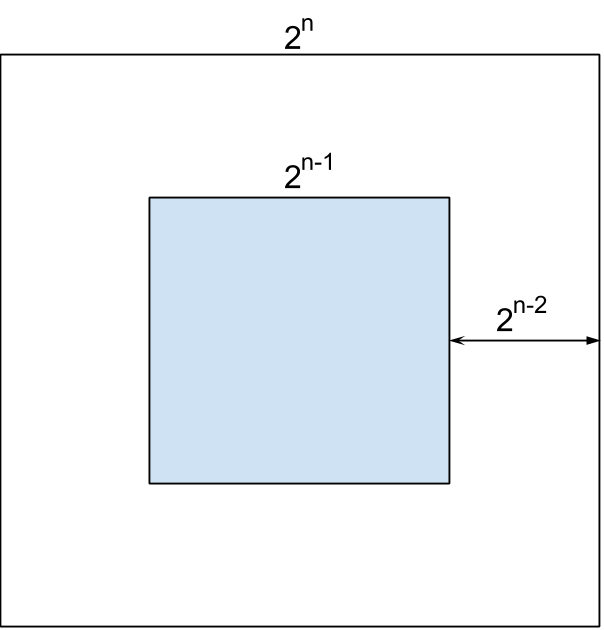
\includegraphics{result.mps}

      \medskip

      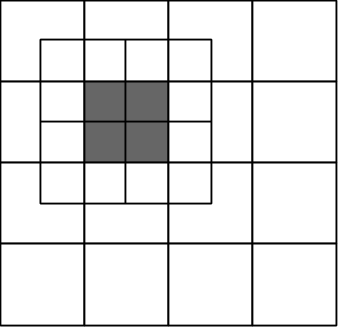
\includegraphics[scale=0.24]{result_3.png}
    \end{column}

    \begin{column}{2cm}
      \includegraphics{result2.mps}

      \medskip

      \includegraphics{result4.mps}
    \end{column}

  \end{columns}

\end{frame}

\subsection{Hash-consing et mémoïsation}

\begin{frame}{Hash-consing et mémoïsation}

\begin{itemize}
\item La mémoïsation permet de ne pas avoir à refaire des
  calculs déjà effectués.
\item Hash-consing : cas particulier visant à mémoïser les
  constructions. 

\bigskip
  Permet d'exploiter la redondance des macro-cellules
\end{itemize}

\end{frame}

\begin{frame}{Démo}
  
\end{frame}

\section{Détails d'implémentation}

\begin{frame}{Architecture du programme}

\begin{figure}
  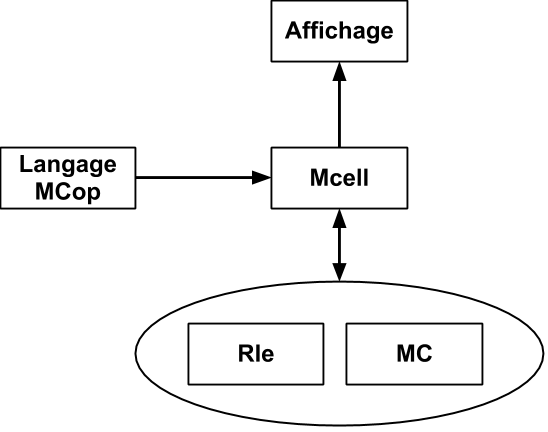
\includegraphics[scale=0.4]{dtech.png}
%  \caption{Architecture du programme}
\end{figure}

\end{frame}

\subsection{Mise en oeuvre du hash-consing}

\begin{frame}[fragile]{Mise en oeuvre du hash-consing}

une macro-cellule :

\begin{verbatim}
  type t = { nw : t, ne : t, sw : t, se : t, 
             result : t, id : int, size : int }
\end{verbatim}

\medskip

principe du hash-consing :

\begin{semiverbatim}
  let create nw ne sw se =
    \textit{crée la macro-cellule (nw,ne,sw,se)
    cherche dans la table de hachage si elle existe déjà
    si oui, renvoie celle de la table
    sinon ajoute celle créée à la table et la renvoie}
\end{semiverbatim}

\end{frame}

\begin{frame}[fragile]{le faire efficacemment}

  la table de hachage utilise les deux opérations
  
\begin{verbatim}
  let equal m1 m2 =
    m1.nw == m2.nw && m1.ne == m2.ne && 
    m1.sw == m2.sw && m1.se == m2.se
      
  let hash m = 
    abs (19 * (19 * 
      (19 * m.nw.id + m.ne.id) + m.sw.id) + m.se.id)
\end{verbatim}

  ces deux opérations ont \alert{un coût $O(1)$}

\end{frame}

\subsection{Affichage de macro-cellules}

\begin{frame}{Affichage de macro-cellules}

  \begin{center}
    Nécessité de \alert{découper} l'affichage

    \medskip

    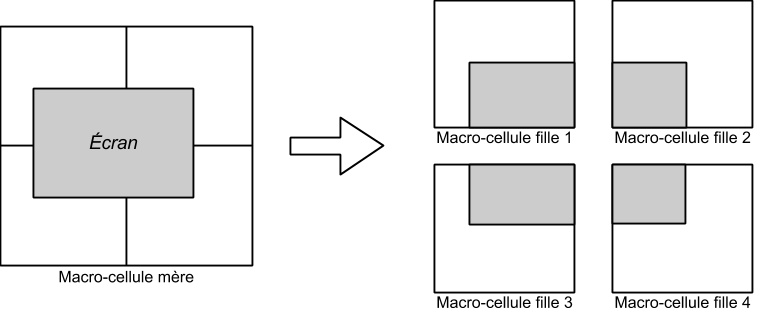
\includegraphics[scale=0.4]{decoupage_graphique.png}
  \end{center}
\end{frame}

\subsection{Parsing des fichiers de description}

\begin{frame}{Parsing des fichiers de description}
  Deux formats possibles de description du Jeu de la Vie
  \begin{itemize}
    \item \textbf{Extended RLE} (\textit{Run-Length Encoding})

      Description linéaire d'une grille

      \medskip

    \item \textbf{MC} (\textit{MacroCells})

      Format exploitant la redondance des configurations

  \end{itemize}
\end{frame}

\subsection{Extensions et langage MCop} 

\begin{frame}{Extensions} 
  Opérations sur les macro-cellules
  \begin{itemize}
    \item Union
    \item Intersection
    \item Différence
    \item Symétrie axiale verticale
    \item Rotation à 90, 180 et 270 degrés
  \end{itemize}

  \medskip

  Chacune de ces opérations est \alert{mémoïsée}

\end{frame}

\begin{frame}[fragile]{Langage de script}
  Langage permettant la manipulation de macro-cellules, qui utilise
  les fonctions introduites précédemment.

  \medskip

  Exemple :
\begin{verbatim}
  let a = extend(extend(readRle("files/puffer.rle"))) in
  let b = union(a, mirror(a)) in
  let c = rotate90(b) in
  let res = union(b, c) in
  outMC(res, "resultat.mc")
\end{verbatim}

\end{frame}

\section{Performances}

\begin{frame}
  \begin{center}
    Évaluation expérimentale
  \end{center}
\end{frame}

\begin{frame}{Performance : expérience 1}
  \begin{figure}
    \centering
    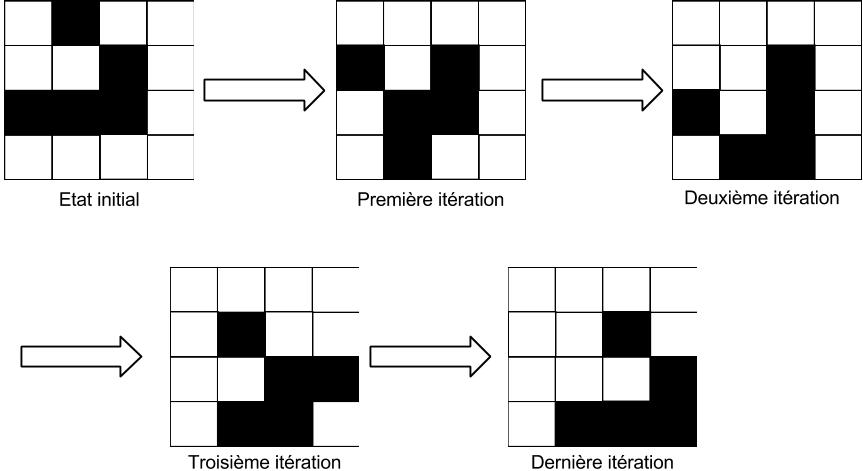
\includegraphics[scale=0.3]{perf_glider_iterations.png}
    \caption{Les itérations du glider}
  \end{figure}
\end{frame}

\begin{frame}{Performance : expérience 1}
  \begin{figure}
    \centering
    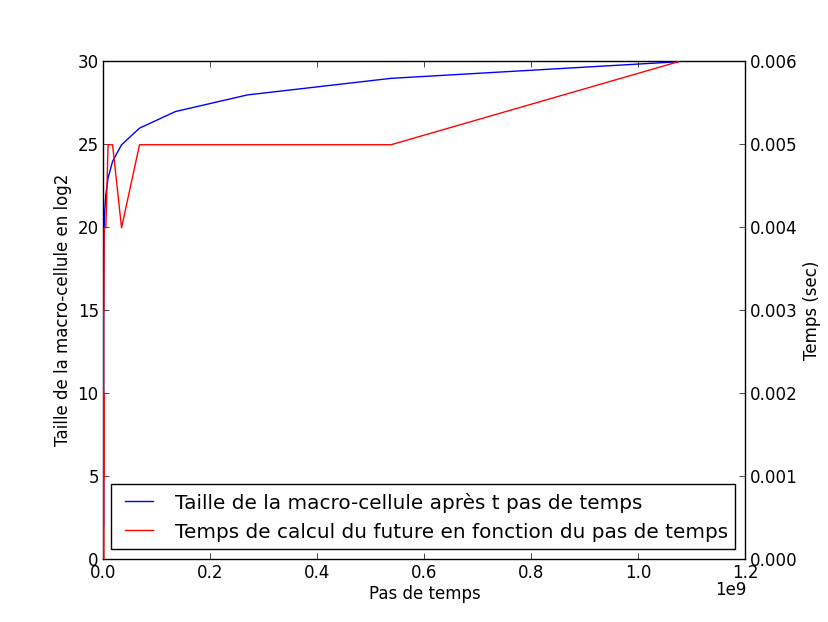
\includegraphics[scale=0.4]{perf_glider_graph.png}
    \caption{Tests sur le glider}
  \end{figure}
\end{frame}

\begin{frame}{Performance : expérience 2}
  \begin{figure}
    \centering
    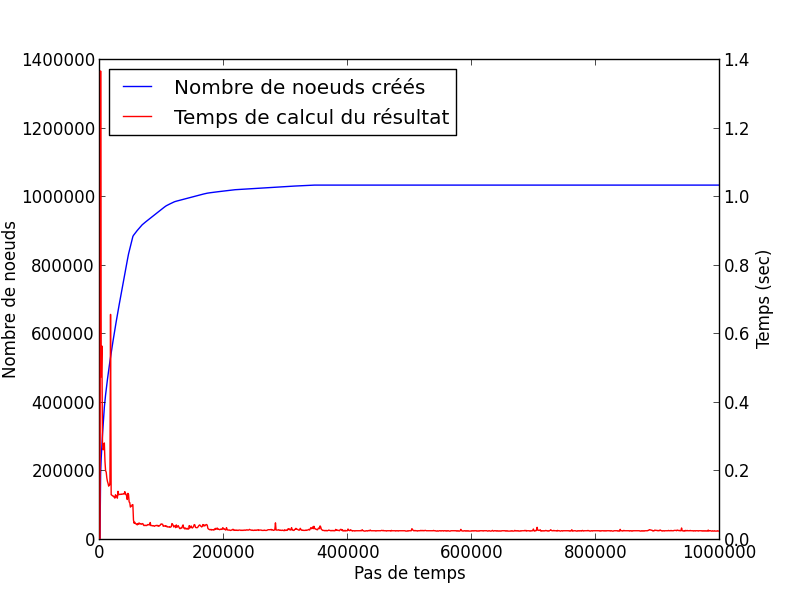
\includegraphics[scale=0.4]{perf_ticker.png}
    \caption{Tests sur le ticker}
  \end{figure}
\end{frame}

\begin{frame}{Performance : expérience 3}
  \begin{columns}[c]
    \begin{column}{5cm}
      \begin{figure}
        \centering
        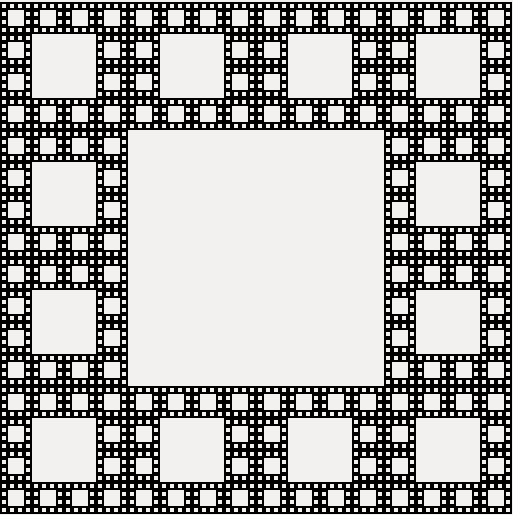
\includegraphics[scale=0.3]{perf_carpet.png}
      \end{figure}
    \end{column}
    \begin{column}{5cm}
      \begin{figure}
        \centering
        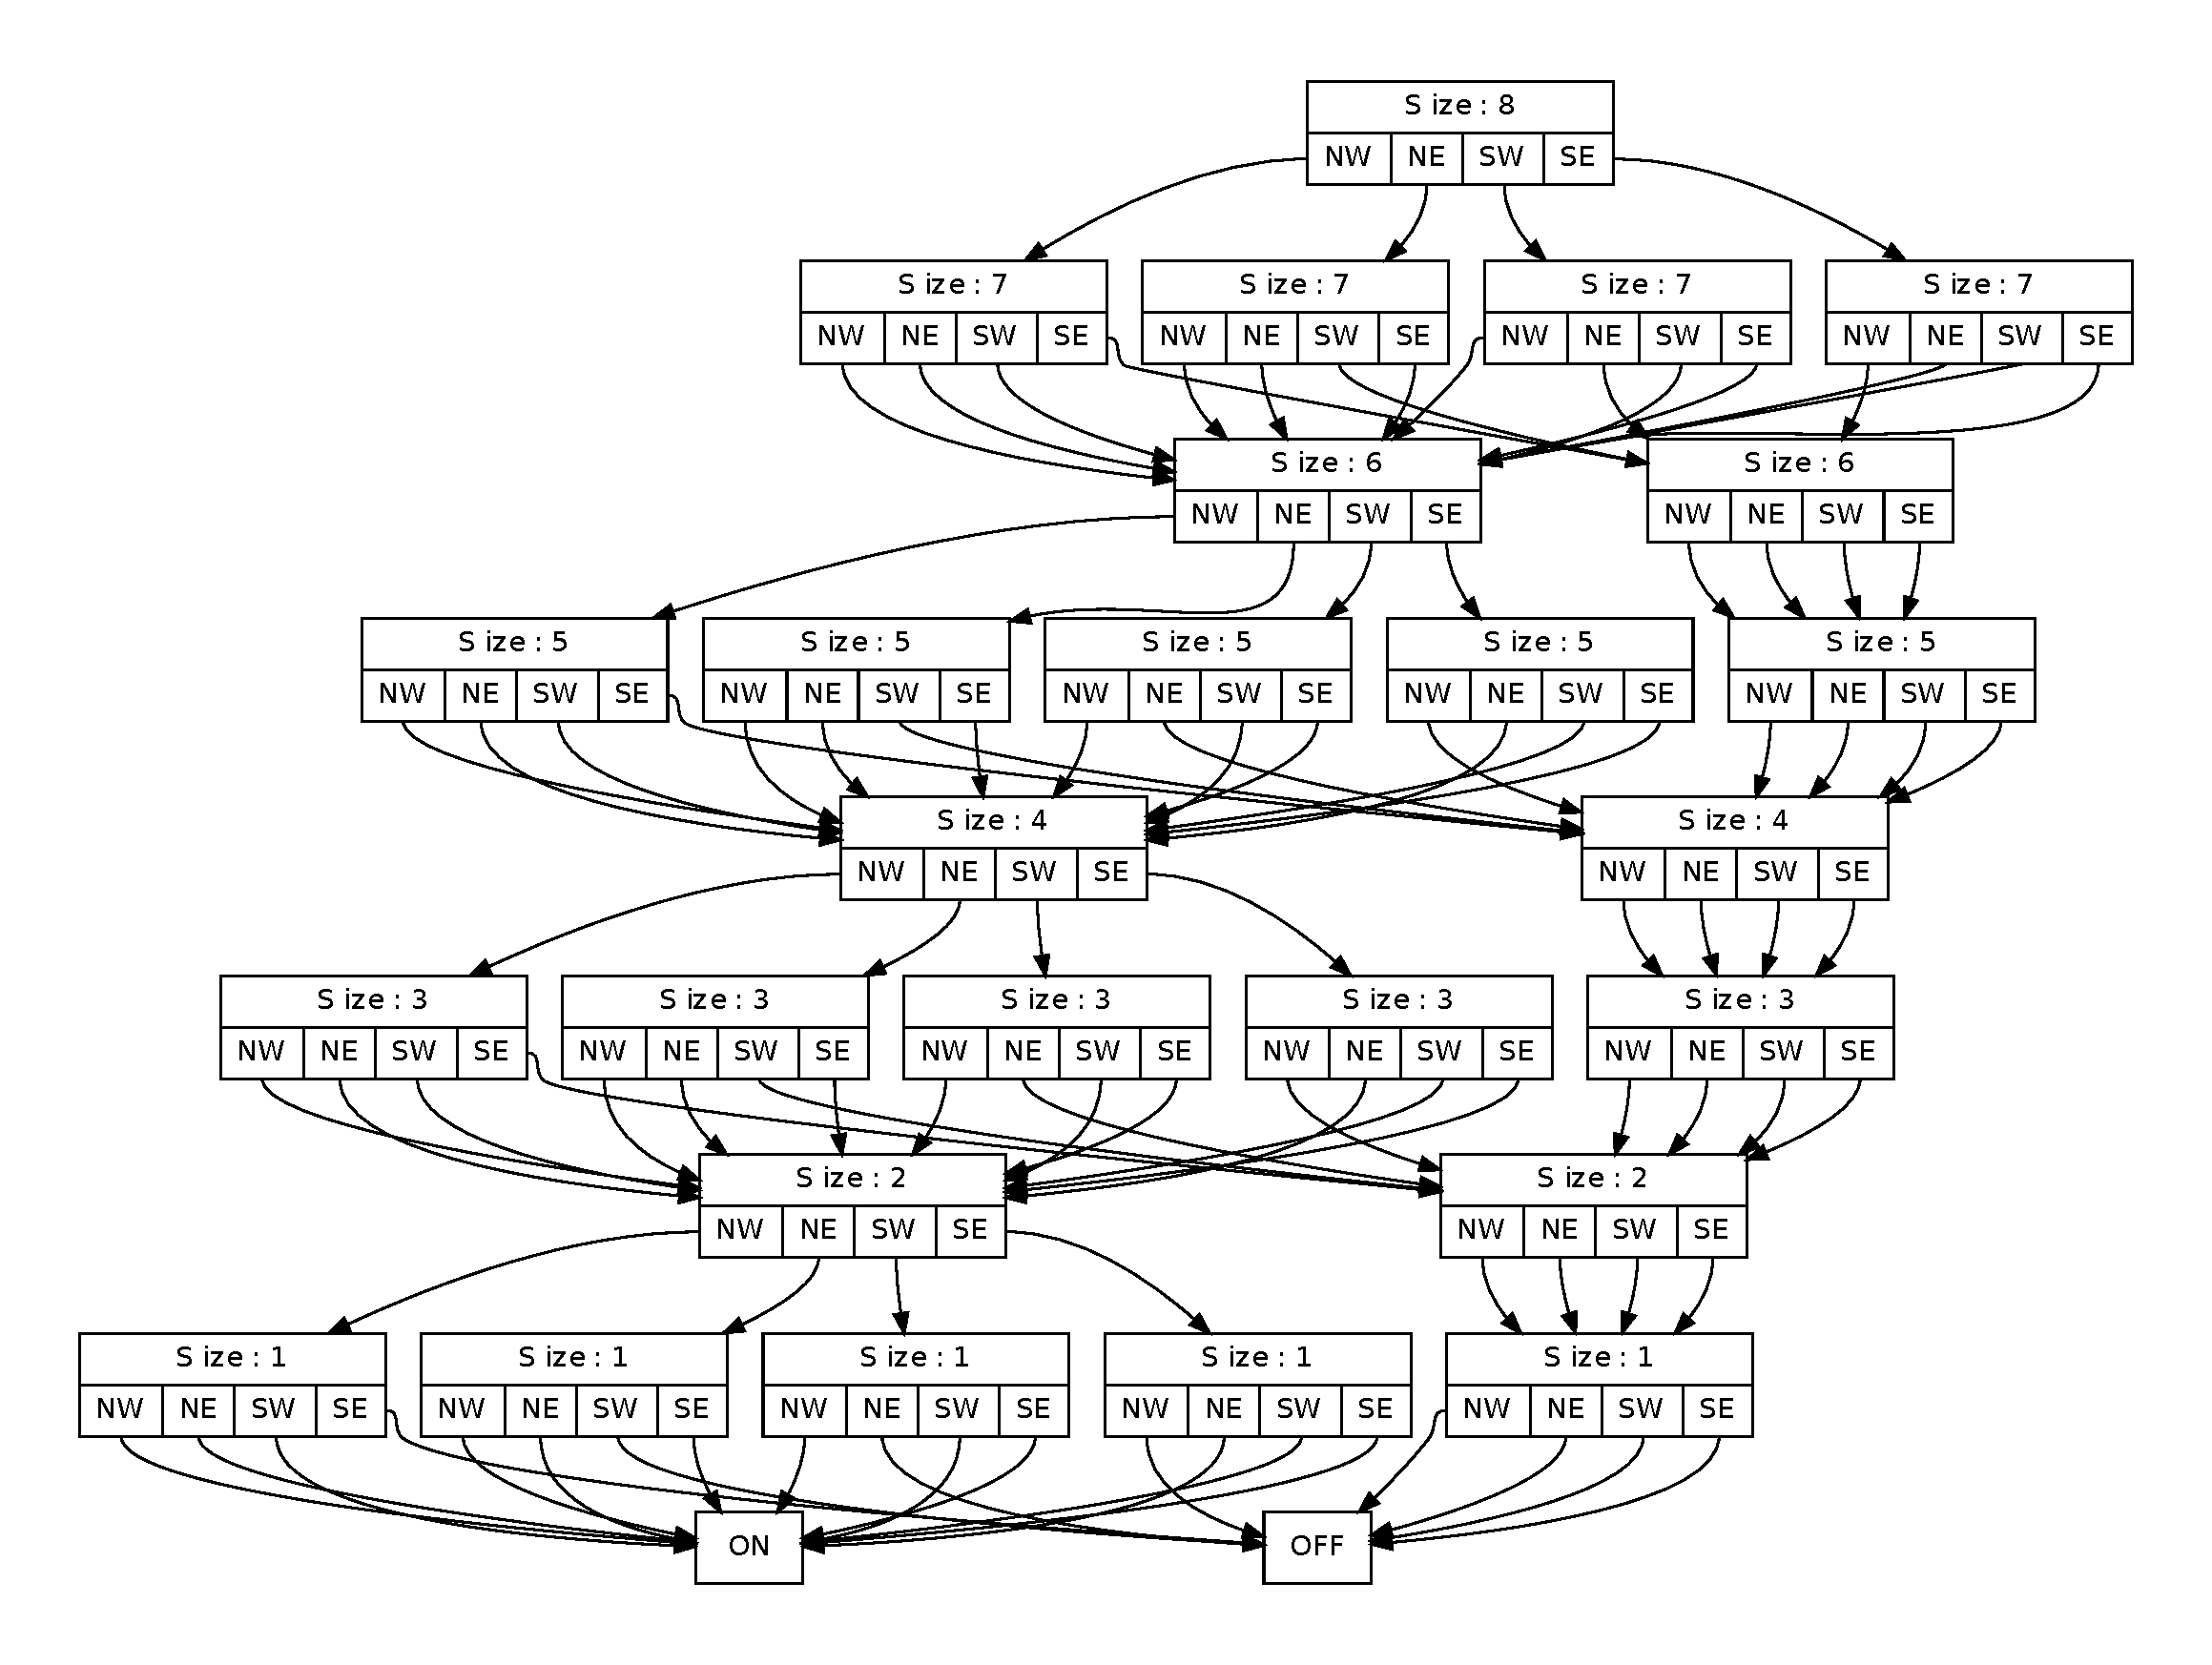
\includegraphics[scale=0.15]{perf_memCarpet.pdf}
      \end{figure}
    \end{column}
  \end{columns}
  \begin{center}
    Tapis de Sierpinski de taille 8 et sa représentation en mémoire
  \end{center}
\end{frame}


\begin{frame}{Performance : expérience 3}
  \begin{figure}
    \centering
    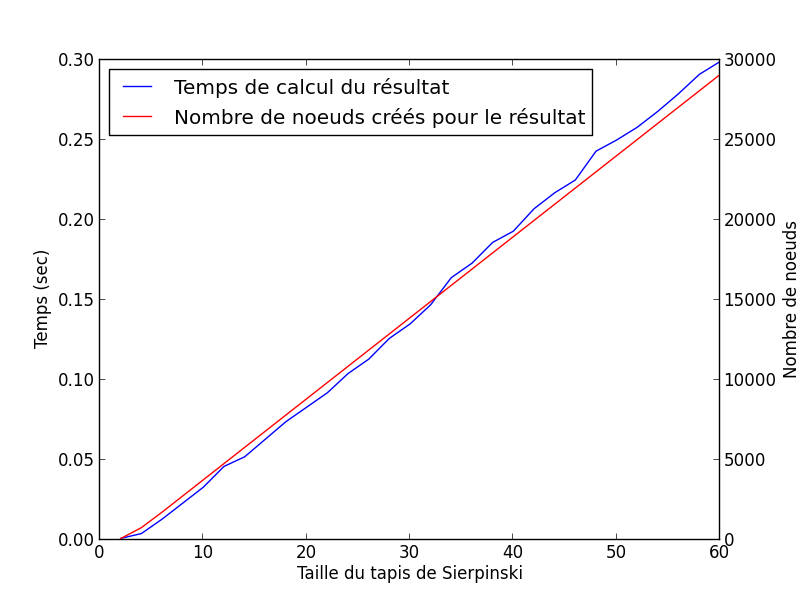
\includegraphics[scale=0.4]{perf_carpet_time_created.png}
    \caption{Tests sur le tapis de Sierpinski}
  \end{figure}
\end{frame}

\begin{frame}{Utilité du TER}
  \begin{itemize}
  \item Hash-consing et mémoïsation réutilisables dans de nombreux contextes
    (exemple : les BDD)
  \item Alternative élégante à la programmation dynamique
  \item Structure de quadtree, qui se retrouve notamment dans un navigateur GPS
    (à la Google Maps)
  \end{itemize}
\end{frame}
 
\end{document}

% Local Variables:
% compile-command: "rubber -d slides.tex"
% ispell-local-dictionary: "francais"
% End:
% LocalWords:  Hashlife quadtree Hash-consing mémoïsation Parsing RLE
% LocalWords:  d'implémentation hash-consing macro-cellules mémoïsées
%  LocalWords:  macro-cellule unaires axiale MacroCells Extended MC
%  LocalWords:  Run-Length Encoding MCop
